\documentclass[aspectratio=169]{beamer}

% ===== Tema: stesso stile del progetto di Apprendimento Automatico =====
\usetheme{Boadilla}
\useinnertheme{rounded}
\setbeamertemplate{blocks}[rounded][shadow=true]
\setbeamertemplate{navigation symbols}{}
\setbeamertemplate{itemize items}[circle]

% Banda chiara dietro il titolo del frame (come nel deck ML)
\setbeamercolor{frametitle}{fg=black, bg=structure!12}
\setbeamertemplate{frametitle}{%
  \nointerlineskip%
  \begin{beamercolorbox}[wd=\paperwidth,sep=0.35cm,leftskip=0.3cm]{frametitle}%
    \usebeamerfont{frametitle}\insertframetitle%
  \end{beamercolorbox}%
  {\color{structure!35}\rule{\paperwidth}{0.4pt}}%
}

\usepackage[utf8]{inputenc}
\usepackage[T1]{fontenc}
\usepackage[italian]{babel}
\usepackage{amsmath, amssymb}
\usepackage{booktabs}
\usepackage{graphicx}
\usepackage{tikz}

\graphicspath{{figure/}}

% ===== Metadati (footer tripartito, come nel deck ML) =====
\title[Progetto DL]{Progetto di Apprendimento Automatico e Profondo}
\subtitle{Object Detection e Sentiment Analysis: da YOLO ai Transformer}
\author{Matteo Barbieri}
\institute[Apprendimento Automatico e Profondo]{Apprendimento Automatico e Profondo}
\date{16 luglio 2026}

% Scaletta all'inizio di ogni sezione (come nel deck ML)
\AtBeginSection[]{%
  \begin{frame}{Scaletta}
    \tableofcontents[currentsection]
  \end{frame}%
}

\begin{document}

% Box arrotordato per il titolo (come nel deck ML)
\setbeamercolor{titlebox}{fg=structure, bg=structure!12}

\begin{frame}[plain]
  \vfill
  \begin{center}
    \begin{beamercolorbox}[rounded=true, shadow=true, wd=0.88\paperwidth,
                           sep=10pt, center]{titlebox}
      {\usebeamerfont{title}\inserttitle}\\[4pt]
      {\usebeamerfont{subtitle}\normalsize\insertsubtitle}
    \end{beamercolorbox}
  \end{center}
  \vspace{0.9cm}
  \begin{center}
    {\usebeamerfont{author}\insertauthor}\\[10pt]
    {\small\insertinstitute}\\[14pt]
    {\insertdate}
  \end{center}
  \vfill
\end{frame}

\begin{frame}{Scaletta}
  \tableofcontents
\end{frame}

% ==================================================================
\section{Introduzione: reti neurali}
% ==================================================================

\begin{frame}{Il neurone}
  \begin{block}{Modello del neurone}
    Il neurone calcola una \textbf{combinazione lineare} degli input e vi applica
    una \textbf{funzione di attivazione} $g$:
    \[ z = \sum_{j=1}^{n} w_j x_j + b , \qquad a = g(z) \]
  \end{block}
  \begin{itemize}
    \item $w_j$ = \textbf{pesi} (quanto conta ogni input), $b$ = \textbf{bias}.
    \item Con il trucco della \emph{bias unit} $x_0=1$ si scrive compattamente
          $z = \theta^{\top}\mathbf{x}$.
    \item Senza $g$ il neurone è solo un \textbf{prodotto scalare}: è $g$ a dare
          la \alert{non linearità}.
  \end{itemize}
\end{frame}

\begin{frame}{Dalla rete al forward propagation}
  I neuroni si organizzano in \textbf{layer}: l'output di un layer è l'input del
  successivo (\emph{forward propagation}):
  \[ \mathbf{a}^{(l)} = g\!\left( W^{(l)} \mathbf{a}^{(l-1)} + \mathbf{b}^{(l)} \right) \]
  \begin{columns}[T]
    \begin{column}{0.5\textwidth}
      \begin{block}{Feature apprese}
        La rete \textbf{scopre da sola} le feature nascoste: la semantica la
        diamo noi. (Es.\ prezzo di una casa: un'unità nascosta può rappresentare
        la ``dimensione della famiglia''.)
      \end{block}
    \end{column}
    \begin{column}{0.5\textwidth}
      \begin{block}{Perché non lineari?}
        Con sole attivazioni \textbf{lineari} una rete profonda equivale a
        \textbf{un solo neurone}. Con attivazioni non lineari diventa un
        \alert{approssimatore universale di funzioni}.
      \end{block}
    \end{column}
  \end{columns}
\end{frame}

\begin{frame}{Funzioni di attivazione}
  \begin{columns}[T]
    \begin{column}{0.52\textwidth}
      \[ \sigma(z)=\frac{1}{1+e^{-z}} \qquad \mathrm{ReLU}(z)=\max(0,z) \]
      \begin{itemize}
        \item \textbf{Layer nascosti}: \textbf{ReLU} (oggi lo standard).
        \item \textbf{Output regressione}: lineare / identità.
        \item \textbf{Output binario}: sigmoide (logistica).
        \item \textbf{Output multiclasse}: \textbf{softmax}.
      \end{itemize}
      \vspace{0.1cm}
      {\footnotesize Il passaggio da \emph{sigmoide} a \emph{ReLU} è uno dei
      progressi algoritmici che hanno reso possibile il deep learning.}
    \end{column}
    \begin{column}{0.48\textwidth}
      \centering
      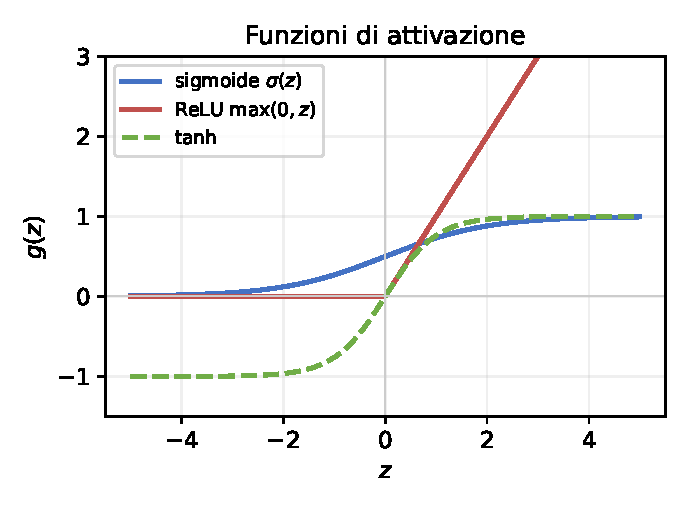
\includegraphics[width=\textwidth]{attivazioni.pdf}
    \end{column}
  \end{columns}
  \vspace{0.1cm}
  \[ \mathrm{softmax}(\mathbf{z})_k=\frac{e^{z_k}}{\sum_j e^{z_j}}
     \quad\text{(la logistica ne è il caso binario)} \]
\end{frame}

\begin{frame}{La funzione di costo}
  La rete produce $\hat{y}$; la \textbf{loss} misura quanto sbaglia su un
  esempio, il \textbf{costo} $J$ è la media su tutti gli $m$ esempi:
  \[ J(\theta)=\frac{1}{m}\sum_{i=1}^{m} L\!\left(\hat{y}^{(i)}, y^{(i)}\right) \]
  \begin{columns}[T]
    \begin{column}{0.5\textwidth}
      \begin{block}{Regressione: errore quadratico}
        \[ L = \tfrac{1}{2}\left(\hat{y}-y\right)^2 \]
        {\footnotesize Il fattore $\tfrac{1}{2}$ semplifica la derivata.}
      \end{block}
    \end{column}
    \begin{column}{0.5\textwidth}
      \begin{block}{Classificazione: cross-entropy}
        \[ L = -\sum_k y_k \log \hat{y}_k \]
      \end{block}
    \end{column}
  \end{columns}
  \vspace{0.2cm}
  {\footnotesize Nel progetto usiamo \textbf{entrambe}: errore quadratico per le
  coordinate delle bounding box, cross-entropy per le classi e il sentiment.}
\end{frame}

\begin{frame}{Apprendimento: gradient descent e backpropagation}
  \begin{block}{Regola di aggiornamento}
    Si aggiornano i parametri nella direzione \textbf{opposta al gradiente}:
    \[ \theta := \theta - \alpha \frac{\partial J}{\partial \theta} \]
    con $\alpha$ = \textbf{learning rate} (ampiezza del passo).
  \end{block}
  \begin{itemize}
    \item Il gradiente si calcola con la \textbf{backpropagation}: si propaga
          l'errore all'indietro applicando la \emph{regola della catena},
          usando la derivata della funzione di attivazione di ogni unità.
    \item $\alpha$ troppo grande $\to$ si diverge; troppo piccolo $\to$
          convergenza lentissima.
  \end{itemize}
\end{frame}

\begin{frame}{Ottimizzazione: dal mini-batch ad Adam}
  \begin{itemize}
    \item \textbf{Mini-batch gradient descent}: aggiornare i pesi usando tutto
          il dataset è proibitivo $\Rightarrow$ si procede a blocchi
          (tipicamente 32--256 esempi). \emph{Nel progetto: batch da 16.}
  \end{itemize}
  \begin{block}{Migliorare la discesa (medie mobili esponenziali)}
    \begin{itemize}
      \item \textbf{Momentum}: media mobile del \emph{gradiente} $\to$ aiuta a
            uscire dai minimi locali e smorza le oscillazioni.
      \item \textbf{RMSprop}: media mobile del \emph{quadrato} del gradiente
            $\to$ normalizza le fluttuazioni dividendo per la sua radice.
      \item \alert{\textbf{Adam}}: combina Momentum e RMSprop, con
            \emph{bias correction}.
    \end{itemize}
  \end{block}
  \begin{center}
    \small Adam è l'ottimizzatore usato in \textbf{entrambi} gli esercizi.
  \end{center}
\end{frame}

\begin{frame}{Batch Normalization}
  \begin{block}{Idea}
    Come si normalizzano gli input, si possono normalizzare anche i valori dei
    \textbf{nodi interni}, usando media e varianza calcolate su ogni
    \textbf{mini-batch} (poi riscalati con parametri apprendibili).
  \end{block}
  \begin{itemize}
    \item Contrasta il \textbf{covariate shift}: i layer profondi ricevono input
          la cui distribuzione cambia di continuo durante il training.
    \item In pratica: si aggiunge un \textbf{layer BN} dopo il layer da
          normalizzare e si fa la solita backpropagation.
    \item A test time si usano le medie mobili accumulate durante il training.
  \end{itemize}
  \begin{center}
    \small Usata in ogni blocco convoluzionale del detector: \texttt{Conv $\to$ BN $\to$ ReLU}.
  \end{center}
\end{frame}

\begin{frame}{Dal neurone al deep learning}
  \begin{block}{Idea del deep learning}
    Comporre (\emph{nesting}) funzioni semplici in una sequenza di layer sempre
    più \textbf{astratti}: le \emph{feature} vengono apprese insieme
    all'obiettivo (\emph{representational learning}).
  \end{block}
  \textbf{Approcci principali del corso}: feedforward, \textbf{CNN} (immagini),
  reti ricorrenti, \textbf{Transformer} (sequenze), autoencoder, GAN.
  \vspace{0.3cm}
  \begin{block}{I due esercizi usano due di questi approcci}
    \begin{itemize}
      \item \textbf{Object detection} $\to$ rete \textbf{convoluzionale} (CNN).
      \item \textbf{Sentiment analysis} $\to$ \textbf{Transformer}.
    \end{itemize}
  \end{block}
\end{frame}

% ==================================================================
\section{Object Detection (YOLO)}
% ==================================================================

\begin{frame}{Reti convoluzionali: la convoluzione}
  \begin{columns}[T]
    \begin{column}{0.5\textwidth}
      Una rete densa su immagini grandi è \textbf{ingestibile} (troppi pesi).
      \vspace{0.2cm}

      La \textbf{convoluzione} fa scorrere un piccolo \textbf{filtro} (kernel)
      sull'immagine, calcolando un prodotto scalare a ogni posizione $\to$
      produce una \emph{feature map}.
      \vspace{0.2cm}
      \begin{block}{Filtri appresi, non progettati}
        Un filtro può rilevare i \textbf{bordi} (verticali, orizzontali).
        Invece di costruirlo a mano (Sobel, Scharr), si \alert{apprendono i pesi
        del filtro} con la backpropagation.
      \end{block}
    \end{column}
    \begin{column}{0.5\textwidth}
      \centering
      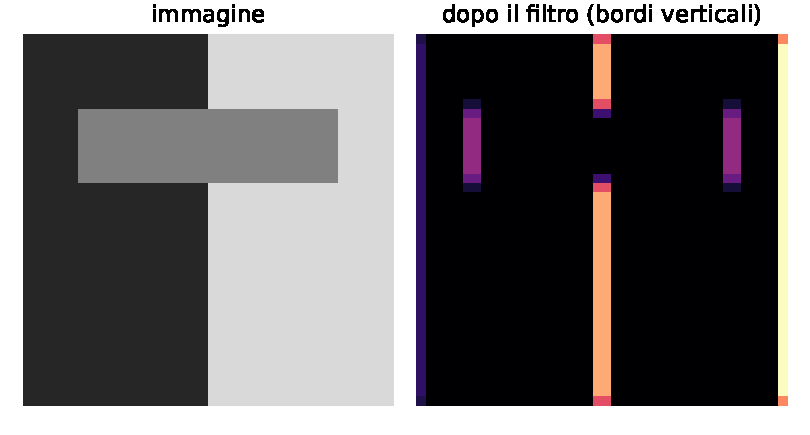
\includegraphics[width=\textwidth]{cnn_edge.pdf}\\[4pt]
      {\footnotesize Un filtro verticale evidenzia i bordi verticali.}
    \end{column}
  \end{columns}
\end{frame}

\begin{frame}{CNN: padding, stride, pooling}
  \begin{columns}[T]
    \begin{column}{0.5\textwidth}
      \begin{block}{Iperparametri della convoluzione}
        \begin{itemize}
          \item \textbf{Padding}: bordo di zeri; \emph{same} mantiene la
                dimensione, \emph{valid} la riduce.
          \item \textbf{Stride}: di quanti passi scorre il filtro.
          \item \textbf{Più filtri} $\to$ più feature map (profondità).
                Su immagini RGB: convoluzione su ogni canale, poi somma.
        \end{itemize}
      \end{block}
    \end{column}
    \begin{column}{0.5\textwidth}
      \begin{block}{Pooling}
        Il \textbf{max pooling} tiene il valore massimo di ogni regione:
        riduce la dimensione e agisce da rilevatore di feature.
      \end{block}
      \vspace{0.1cm}
      \textbf{Architettura tipica}:
      \[ \text{CONV} \to \text{POOL} \to \dots \to \text{FC} \]
      Andando in profondità: più filtri, dimensioni spaziali più piccole.
    \end{column}
  \end{columns}
\end{frame}

\begin{frame}{Perché la convoluzione funziona}
  \begin{block}{Due proprietà chiave}
    \begin{itemize}
      \item \textbf{Parameter sharing}: un rilevatore di feature (es.\ un bordo)
            è utile in \textbf{tutta} l'immagine $\to$ pochissimi parametri, che
            \emph{non dipendono} dalla dimensione dell'immagine.
      \item \textbf{Sparsità delle connessioni}: ogni output dipende solo da una
            \textbf{piccola regione} dell'input $\to$ meno parametri, meno
            overfitting.
    \end{itemize}
  \end{block}
  \begin{center}
    \small Nel detector: 5 blocchi \texttt{Conv $\to$ BN $\to$ ReLU} + max-pool
    riducono $224\times224$ fino alla griglia $7\times7$.
  \end{center}
\end{frame}

\begin{frame}{Il problema: localizzazione con bounding box}
  \begin{block}{Object detection}
    Data un'immagine, individuare \textbf{quali} oggetti contiene e \textbf{dove}
    si trovano, disegnando una \emph{bounding box} attorno a ciascuno.
  \end{block}
  \vspace{0.3cm}
  \textbf{Dataset: Object365} (365 classi, 600k immagini, 10M box).
  \begin{itemize}
    \item Volume incompatibile con un portatile $\Rightarrow$ \alert{subsampling} su due assi.
    \item \textbf{Classi}: da 365 a \textbf{8} frequenti (Person, Car, Chair, Bottle, Cup, Lamp, Hat, Book).
    \item \textbf{Immagini}: 4.867 tenute (50.071 box); solo quelle con almeno un oggetto utile.
  \end{itemize}
  \begin{center}
    \small Tecnica scelta: \textbf{YOLO}. Griglia, anchor, loss, IoU e NMS sono
    \emph{implementati a mano} (nessuna libreria di detection).
  \end{center}
\end{frame}

\begin{frame}{Dalla sliding window a YOLO}
  \begin{columns}[T]
    \begin{column}{0.54\textwidth}
      \textbf{Sliding window}: si fa scorrere una finestra e si classifica ogni ritaglio.
      \begin{itemize}
        \item Problema principale: \alert{costo computazionale}.
        \item Soluzione: implementarla \textbf{convoluzionalmente}.
      \end{itemize}
      \vspace{0.2cm}
      \textbf{YOLO}: griglia $S\times S$; ogni oggetto assegnato a \textbf{una cella}
      (quella del suo centro), che ne predice box e classe.
    \end{column}
    \begin{column}{0.44\textwidth}
      \begin{block}{Anchor box}
        Per ogni cella, $n$ forme predefinite. Se più oggetti cadono nella stessa
        cella, ognuno va all'anchor più simile per forma (IoU).
      \end{block}
      \centering
      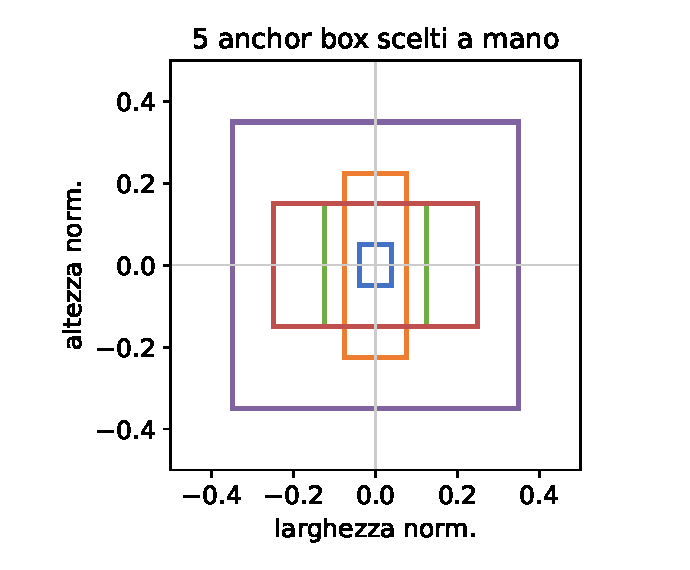
\includegraphics[width=0.86\textwidth]{anchor.pdf}
    \end{column}
  \end{columns}
\end{frame}

\begin{frame}{Distribuzione del dataset}
  \begin{columns}[T]
    \begin{column}{0.46\textwidth}
      \vspace{0.5cm}
      Sottoinsieme fortemente \textbf{sbilanciato}:
      \begin{itemize}
        \item \textbf{Person} da sola: 49,9\% delle box.
        \item \textbf{Book}: appena 2,6\%.
      \end{itemize}
      \vspace{0.2cm}
      $\Rightarrow$ prestazioni attese \alert{inferiori sulle classi rare}.
      \vspace{0.2cm}

      Gli anchor box sono \textbf{scelti a mano} (come indicano le slide),
      a coprire forme tipiche: piccolo, medio, alto, largo, grande.
      \vspace{0.2cm}

      \textbf{Data augmentation} (in training): \textbf{flip orizzontale} (che
      ribalta anche le box, $c_x\!\to\!1-c_x$) + leggero \textbf{color jitter}.
    \end{column}
    \begin{column}{0.54\textwidth}
      \centering
      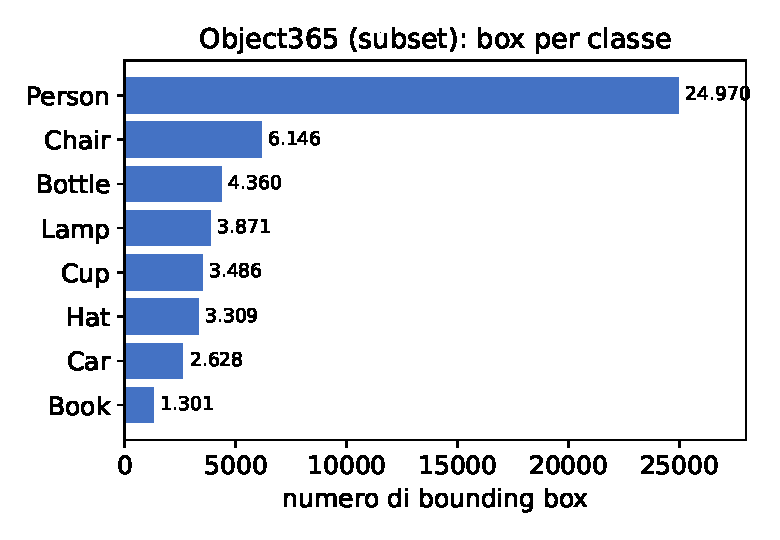
\includegraphics[width=\textwidth]{classi.pdf}
    \end{column}
  \end{columns}
\end{frame}

\begin{frame}[fragile]{Architettura della rete}
  Backbone convoluzionale con downsampling $\times 32$, seguito da una
  \textbf{testa di detection} $1\times1$ scritta da noi.
  \begin{columns}[T]
    \begin{column}{0.52\textwidth}
      {\footnotesize
      \begin{semiverbatim}
Input  3 x 224 x 224
  Backbone (downsampling x32)
             -> 512 x 7 x 7   (griglia S)
  Head 1x1  -> A*(5+C) = 65 canali
Output (5, 7, 7, 13)
      \end{semiverbatim}}
      \vspace{0.1cm}
      \begin{itemize}
        \item Rete \textbf{completamente convoluzionale}.
        \item \textbf{245} box candidate per immagine ($5\times7\times7$).
      \end{itemize}
    \end{column}
    \begin{column}{0.46\textwidth}
      \begin{block}{Due backbone a confronto}
        \begin{itemize}
          \item \textbf{Da zero}: Conv--BN--ReLU + max-pool (15,8M par.).
          \item \alert{\textbf{ResNet18 pre-addestrata}} su ImageNet, poi
                fine-tunata (11,2M par.) --- \emph{transfer learning}.
        \end{itemize}
      \end{block}
      {\footnotesize In entrambi i casi anchor, target, loss, IoU e NMS
      restano \textbf{implementati a mano}: cambia solo l'estrattore di feature.}
    \end{column}
  \end{columns}
\end{frame}

\begin{frame}{La loss YOLO}
  La rete predice \emph{logit grezzi}, decodificati come (YOLOv2):
  \[
    b_x=\sigma(t_x)+c_x,\quad b_y=\sigma(t_y)+c_y,\quad
    b_w=a_w e^{t_w},\quad b_h=a_h e^{t_h}
  \]
  \begin{block}{Quattro componenti (normalizzate per numero di oggetti)}
    \centering
    \begin{tabular}{llll}
      \toprule
      Componente & Funzione & Peso & Si applica a \\
      \midrule
      Coordinate & MSE & $\lambda=5$ & anchor responsabili \\
      Objectness & BCE & $1$ & anchor responsabili \\
      No-object & BCE & $\lambda=0{,}5$ & anchor non responsabili \\
      Classe & Cross-entropy & $1$ & anchor responsabili \\
      \bottomrule
    \end{tabular}
  \end{block}
  Pesi asimmetrici: su 245 box quasi tutte sono vuote $\Rightarrow$ evitano la
  soluzione degenere \alert{``non c'è mai niente''}.
\end{frame}

\begin{frame}{Inferenza: non-max suppression}
  \begin{columns}[T]
    \begin{column}{0.5\textwidth}
      Ogni box: \textbf{score} $=$ objectness $\times$ prob.\ classe.
      \begin{enumerate}
        \item Scarta le box sotto soglia (0,25).
        \item \textbf{NMS} per classe.
      \end{enumerate}
    \end{column}
    \begin{column}{0.5\textwidth}
      \begin{block}{Non-max suppression}
        {\footnotesize
        ordina le box per score\\
        finché restano box:\\
        \quad prendi quella con score max $\to$ predizione\\
        \quad scarta le altre con $\text{IoU}>$ soglia}
      \end{block}
    \end{column}
  \end{columns}
  \vspace{0.2cm}
  NMS \emph{per classe}: due oggetti di classi diverse possono sovrapporsi (una
  persona con un cappello); due box sovrapposte della stessa classe no.
\end{frame}

\begin{frame}{Valutazione e ottimizzazione dei tempi}
  \begin{columns}[T]
    \begin{column}{0.5\textwidth}
      \textbf{Metrica}: \textbf{precision} e \textbf{recall} a IoU $\geq 0{,}5$
      (l'IoU \`e la misura del corso), implementata a mano. Niente mAP.
      \vspace{0.2cm}
      \begin{alertblock}{Stato del training}
        Il training finale \textbf{non è ancora stato completato}:
        nessun valore di precision/recall disponibile. Tutti i componenti
        sono però implementati e verificati.
      \end{alertblock}
    \end{column}
    \begin{column}{0.5\textwidth}
      \centering
      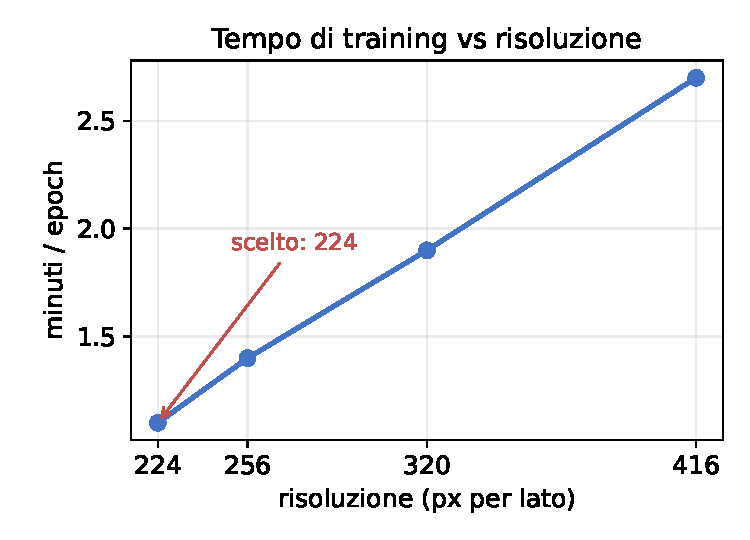
\includegraphics[width=\textwidth]{tempi.pdf}\\
      {\footnotesize Ridurre la risoluzione dimezza i tempi;
      scelto $224$ ($\sim$23 min).}
    \end{column}
  \end{columns}
\end{frame}

% ==================================================================
\section{Sentiment Analysis (Transformer)}
% ==================================================================

\begin{frame}{Il problema: classificare frasi}
  \begin{block}{Sentiment analysis}
    Classificare una sequenza testuale come \textbf{positiva} o \textbf{negativa},
    usando un'architettura \textbf{transformer}.
  \end{block}
  \vspace{0.3cm}
  \begin{itemize}
    \item \textbf{Dataset}: SST-2 (frasi brevi etichettate pos/neg, da HuggingFace).
    \item Corrisponde alla traccia (``frasi positive o negative''); nessun token Kaggle richiesto.
    \item Valutazione sul \emph{validation set} (872 frasi mai viste).
  \end{itemize}
  \begin{center}
    \small Il codice supporta comunque un CSV Kaggle via \texttt{-{}-dataset csv}.
  \end{center}
\end{frame}

\begin{frame}{Dai limiti delle RNN all'attention}
  \textbf{Le RNN} codificano bene la storia recente, ma faticano su contesti
  lontani e sono \textbf{sequenziali} (lente).
  \begin{block}{Esempio delle slide}
    \emph{``I grew up in France, \dots\ thus I speak ??''} --- la parola da predire
    (\emph{French}) dipende da un termine molto \textbf{lontano} nella sequenza.
  \end{block}
  \vspace{0.2cm}
  La risposta è il \textbf{meccanismo di attention}: per produrre la
  rappresentazione di una parola, la si mette in relazione con \textbf{tutte} le
  altre e si pesa quali sono rilevanti, indipendentemente dalla distanza.
\end{frame}

\begin{frame}{Self-attention}
  \begin{columns}[T]
    \begin{column}{0.52\textwidth}
      L'output per ogni parola è una \textbf{somma pesata} delle rappresentazioni
      di tutte le parole; i pesi misurano quanto ognuna è \emph{rilevante}.
      \begin{block}{Proprietà (dalle slide)}
        \begin{itemize}
          \item Calcolo \textbf{parallelo} di tutti gli output (non sequenziale).
          \item \emph{Permutation equivariant}: è più un modello di
                \textbf{insiemi} che di sequenze $\Rightarrow$ serve il
                \textbf{positional encoding} per reintrodurre l'ordine.
        \end{itemize}
      \end{block}
    \end{column}
    \begin{column}{0.48\textwidth}
      \centering
      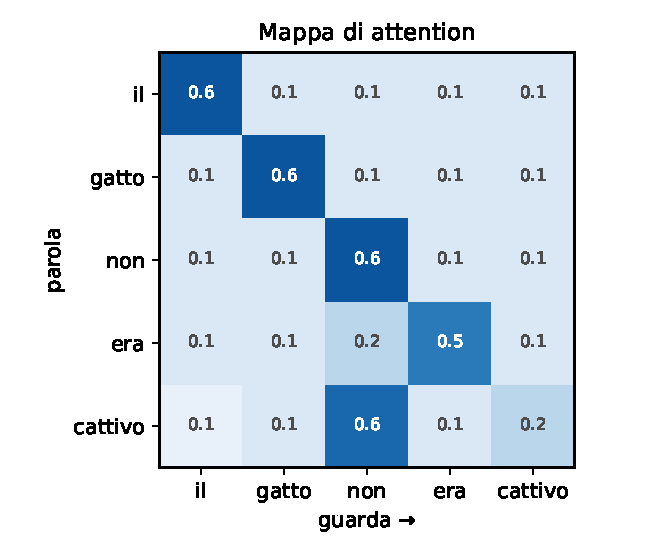
\includegraphics[width=0.92\textwidth]{attention.pdf}\\[3pt]
      {\footnotesize \emph{cattivo} mette attenzione su \emph{non}.}
    \end{column}
  \end{columns}
\end{frame}

\begin{frame}{Query, Key, Value e multi-head}
  \begin{block}{Tre ruoli, tre proiezioni lineari apprese}
    \begin{itemize}
      \item \textbf{Query}: il vettore che viene confrontato con tutti gli altri.
      \item \textbf{Key}: il vettore contro cui la query è confrontata.
      \item \textbf{Value}: ciò che si somma (pesato) per formare l'output.
    \end{itemize}
  \end{block}
  \[ \mathrm{Attention}(Q,K,V)=\mathrm{softmax}\!\left(\frac{QK^{\top}}{\sqrt{d}}\right)V \]
  \begin{itemize}
    \item Divisione per $\sqrt{d}$: \textbf{scaled} attention (stabilità).
    \item \textbf{Multi-head}: più ``teste'' in parallelo, ciascuna cattura un
          tipo diverso di relazione tra le parole.
  \end{itemize}
\end{frame}

\begin{frame}{Il blocco Transformer}
  \begin{columns}[T]
    \begin{column}{0.54\textwidth}
      \begin{block}{Un blocco impila due sotto-strati}
        \begin{enumerate}
          \item \textbf{Multi-head self-attention}
          \item \textbf{Rete feed-forward} (applicata a ogni posizione)
        \end{enumerate}
        Ciascuno con una \textbf{connessione residua} (skip) e una
        \textbf{layer normalization}:
        \[ \mathrm{LayerNorm}\big(x + \mathrm{Sublayer}(x)\big) \]
      \end{block}
      Impilando più blocchi si ottiene il Transformer.
    \end{column}
    \begin{column}{0.46\textwidth}
      \begin{block}{Positional encoding}
        La self-attention è \emph{permutation equivariant}: si \textbf{somma} a
        ogni token un vettore che ne codifica la \textbf{posizione}, così il
        modello conosce l'ordine.
      \end{block}
      \begin{block}{Layer normalization}
        Come la batch norm, ma normalizza sulle \textbf{feature di ogni token}
        (non sul batch).
      \end{block}
    \end{column}
  \end{columns}
\end{frame}

\begin{frame}{Il Transformer e BERT}
  \begin{block}{Transformer}
    Un modello che usa principalmente la \textbf{self-attention} per propagare
    l'informazione tra le unità (token di testo, ma anche pixel: Vision
    Transformer).
  \end{block}
  \begin{columns}[T]
    \begin{column}{0.5\textwidth}
      \textbf{BERT}: transformer \textbf{encoder-only} \emph{bidirezionale},
      pre-addestrato con il \textbf{masking} (predire token nascosti).
      Adatto a \emph{comprendere} una frase, non a generarla.
    \end{column}
    \begin{column}{0.5\textwidth}
      \begin{block}{Il nostro uso}
        \textbf{Fine-tuning} (transfer learning): si parte da BERT
        pre-addestrato e si aggiunge una testa di classificazione binaria.
        Modello: \textbf{DistilBERT}, un BERT più leggero.
      \end{block}
    \end{column}
  \end{columns}
\end{frame}

\begin{frame}{Risultati}
  \begin{columns}[T]
    \begin{column}{0.5\textwidth}
      Fine-tuning su MPS ($\sim$18 min). Metriche sul validation set:
      \vspace{0.2cm}
      \begin{center}
      \begin{tabular}{lr}
        \toprule
        Metrica & Valore \\
        \midrule
        Accuracy & \textbf{89,9\%} \\
        F1 & \textbf{0,901} \\
        Precision & 0,897 \\
        Recall & 0,905 \\
        \bottomrule
      \end{tabular}
      \end{center}
      \vspace{0.2cm}
      Errori \textbf{bilanciati} (46 vs 42): nessun bias di classe.
    \end{column}
    \begin{column}{0.5\textwidth}
      \centering
      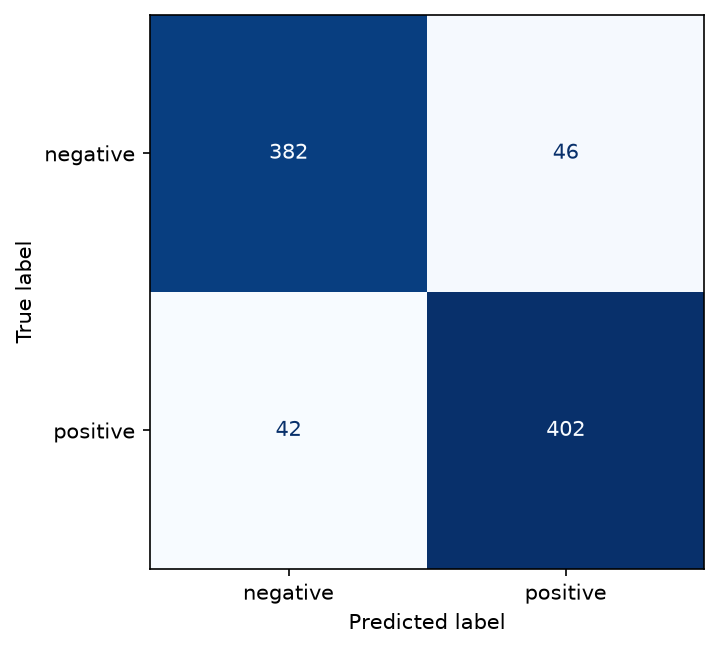
\includegraphics[width=0.92\textwidth]{confusion_matrix.png}
    \end{column}
  \end{columns}
\end{frame}

\begin{frame}{Analisi qualitativa: il caso della negazione}
  Frasi costruite ad hoc:
  \begin{block}{Output del modello}
    {\footnotesize\ttfamily
    {}[positive~~99.9\%] I absolutely loved this film\\
    {}[negative~~99.4\%] the worst purchase I have ever made\\
    {}[positive~~99.9\%] It is not bad at all, quite enjoyable\\
    {}[negative~~69.3\%] predictable but the acting saved it}
  \end{block}
  \begin{itemize}
    \item \emph{``not bad''}: contiene \emph{bad} ma è classificata \textbf{positiva} al 99,9\%.
          L'attention collega \emph{bad} a \emph{not} --- è l'\alert{esempio della slide 11}.
    \item Frase ambigua $\Rightarrow$ confidenza bassa (69\%): il modello \emph{segnala} l'incertezza.
  \end{itemize}
\end{frame}

% ==================================================================
\section{Conclusioni}
% ==================================================================

\begin{frame}{Bilancio}
  \begin{center}
  \begin{tabular}{lll}
    \toprule
     & Esercizio 1 --- Detection & Esercizio 2 --- Sentiment \\
    \midrule
    Codice & Completo (869 righe) & Completo (412 righe) \\
    Pipeline verificata & Si', end-to-end & Si', end-to-end \\
    Modello addestrato & \alert{No} & Si' \\
    Risultati & Non disponibili & Acc.\ 89,9\% --- F1 0,901 \\
    \bottomrule
  \end{tabular}
  \end{center}
  \vspace{0.3cm}
  \begin{itemize}
    \item \textbf{Es.\ 2 concluso}: risultati solidi, allineati a DistilBERT su SST-2.
    \item \textbf{Es.\ 1 completo nell'implementazione}, ma manca il training finale ($\sim$23 min).
  \end{itemize}
\end{frame}

\begin{frame}{Aderenza al programma del corso}
  Il progetto usa \textbf{solo tecniche viste a lezione}: YOLO, anchor, IoU, NMS;
  CNN; \textbf{transfer learning} (backbone ResNet18 pre-addestrato, fine-tuning
  di BERT); transformer, self-attention; Adam, batch norm; data augmentation.
  \begin{block}{Rimosso perch\'e non nel corso $\to$ sostituito}
    \begin{itemize}
      \item anchor k-means $\to$ \textbf{anchor scelti a mano}
      \item meccanismo di ``ignore'' $\to$ rimosso
      \item metrica mAP $\to$ \textbf{precision/recall a IoU $\geq 0{,}5$}
      \item LeakyReLU $\to$ \textbf{ReLU}; cosine + gradient clipping $\to$ rimossi
    \end{itemize}
  \end{block}
  \begin{center}
    \small Mantenuti solo i dettagli \textbf{essenziali} (senza cui i modelli non
    convergono): parametrizzazione sigmoid/exp e pesi $\lambda$ della loss;
    encoder BERT pre-addestrato + tokenizer.
  \end{center}
\end{frame}

\begin{frame}[plain]
  \begin{center}
    {\Large\structure{Grazie per l'attenzione}}\\[0.6cm]
    {\normalsize Matteo Barbieri --- Progetto di Apprendimento Automatico e Profondo}\\[0.2cm]
    {\small Object Detection \& Sentiment Analysis}
  \end{center}
\end{frame}

\end{document}
